\section{Ereditarietà e composizione}

Generalmentesi tende a favorire la composizione in favore dell’eredirarietà.L’ereditarierà e l’override di metodi può essere pericoloso e più difficile di quanto ci si aspetti, proprio come accade per il metodo equals. La cosiddetta tecnica di composizione ci può salvare da questi pericoli:

\begin{lstlisting}
/*ereditarietà*/
public class Test extends Another{
	//codice...
}

/*composizione*/
public class Test {
	private Another a = ... ;
	//codice...
}
\end{lstlisting}
In pratica al posto di ereditare e fare override di metodi si usa un campo privato interno alla classe e si usa quell’oggetto all’interno di alcuni metodi che andranno definiti nella classe contenitore, in questo caso la Test.Vediamo un esempiodove si crea una classe che ne estende un’altra e ha lo scopo di contare quanti elementi sono stati inseriti.

\begin{figure}[H]
\centering
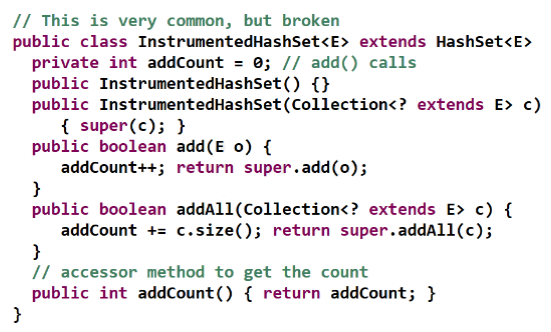
\includegraphics[scale=0.8]{images/composizione}
\caption{Ereditarietà esempio errato\label{fig:UC3}}
\end{figure}
Internamente la classe HashSet implementa addAll()basandosi su add(); in altre parole, la classe HashSet dentro al metodo addAll()chiama add(). Facendo così il metodo addCount() ritorna un numero sbagliato.
\begin{itemize}
	\item La chiamata addAll() incrementa correttamente la variabile addCount ma poi fa una chiamata a super.addAll(c);questo chiama il metodo add()che oltre a chiamare (giustamente) super.add(c);chiama anche addCount++! Quindi il conteggio totale viene sballato perché incremento addCountdi c.size()e poi anche di 1 col ++ ma non dovrei.
	\end{itemize}
	Vediamo dunque che in questo caso possiamo “favor compisition over inheritance” per risolvere il tutto:

	\begin{figure}[H]
\centering
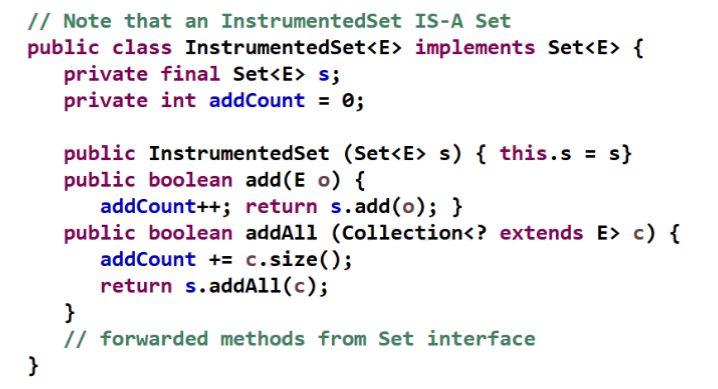
\includegraphics[scale=0.8]{images/composizione2}
\caption{Composizione esempio giusto\label{fig:UC3}}
\end{figure}
Adesso il problema non c’è più perché, avendo un oggetto interno, posso usare questo e non ho bisogno di fare override o fare chiamate a super. Implemento solamente l’interfaccia e faccio override dei contratti dei metodi specificati da quell’interfaccia (Set<E>).